\section{Bluetooth Low Energy}
\label{sec:ble}

Bluetooth is a wireless technology that was created in 1994 with the objective of replacing cables connecting fixed or portable devices. At this point in time Bluetooth Special Interest Group is in charge of developing and managing this technology characterised by its robustness, low energy consumption and low cost. 

The \ac{BLE} protocol was introduced with the Bluetooth Core Specification version 4 (also called Bluetooth Smart) circa 2010 alongside two other protocols.  Out of the three, \ac{BLE} stood out for its lower power consumption, lower complexity and lower cost, while allowing for  device discovery, connection establishment and connection mechanisms. Due to its characteristics, the \ac{BLE} protocol was utilised in various \ac{IoT} applications.  

\subsection{\ac{BLE}'s Architecture}
\label{subsec:BLEArchitecture}

Bluetooth's Architecture is ever-changing and can become very complex rather quickly with the introduction of different types of protocols.
 When working with \ac{BLE} it's important to understand the key components of its architecture  because by doing it's possible to better analyse the role of each component and how they operate and depend on each other. There are two main groups of core blocks, the \ac{LE} Controller and the \ac{LE} Host, in \ref{subsec:LEController} and \ref{subsec:LEHost} respectively, and most the most relevant of these components will now be looked at.
 
 \begin{figure}[H]
	\centering
		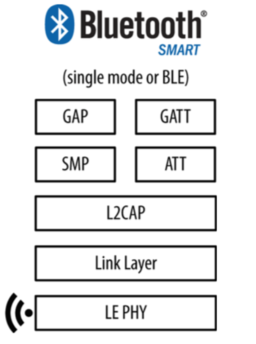
\includegraphics[width=0.5\linewidth]{2.Chapter/BLEArchitecture.png}
	\caption[\ac{BLE} Architecture]{\ac{BLE} architecture}
	\label{fig:BLEarchitecture}
\end{figure}

\subsubsection{ \ac{LE} Controller Group}
\label{subsec:LEController}

\textbf{\ac{PHY} Layer -} Architectural block responsible for all Bluetooth’s communication channels on the 2,4GHz radio. Receiving and transmitting packets and supplying information crucial for controlling its timing and frequency through the baseband block.


\textbf{Link Layer -} Architectural block responsible for managing logical links between \ac{BLE} devices. It can create and release connections, update connection parameters related to \ac{PHY} links. It's responsible for the discovery and consequently connection procedure and also sending and receiving data.


\textbf{Device Manager -} Architectural block responsible for controlling the general behaviour of the Bluetooth device. This block is responsible for all operations that aren't directly related to data transportation. Some of its operations are: inquiring for the presence of nearby  \ac{BLE} devices; connecting to a \ac{BLE} device; setting whether or not its local device is discoverable and/or connectable by the others; controlling device behaviour such as managing own's local name or stored keys. 


\textbf{Baseband Resource Manager -} Architectural block responsible for all access to the radio medium, this means access to the \ac{PHY} channels. It has two purposes, first to negotiate contracts with the entities that wish to use the medium and second to act as a scheduler on the same radio medium, granting the entities with said contracts, a time window in which they can utilise the medium. A contract is basically a commitment to deliver a certain \ac{QoS} on the user application.


\textbf{Link Controller -} Architectural block responsible for the encoding and decoding of Bluetooth packets from the data payload and parameters related to the physical channel, logical transport and logical link. It also carries out the Link Layer protocol in conjunction with Baseband manager's scheduling function to communicate flow control and acknowledgement and retransmission request signals.



\subsubsection{ \ac{LE} Host Group}
\label{subsec:LEHost}

\textbf{\ac{L2CAP} -} Architectural block responsible of transmits packets to the \ac{HCI} or directly to the Link Layer in host-less systems. It allows for higher-level protocol multiplexing, packet segmentation and reassembly, and the conveying of \ac{QoS} information to higher layers.

 
\textbf{Channel Manager -} Architectural block responsible for creating, managing and closing \ac{L2CAP} channels used in transport of service protocols and application data streams. The local Channel Manager makes use of the \ac{L2CAP} protocol to communicate with a peer's Channel Manager and together create \ac{L2CAP} channels and connect their endpoints to the appropriate entities.


\textbf{\ac{SMP} -} Architectural block responsible for implementing the \ac{P2P} protocol that operates over its own dedicated \ac{L2CAP} channel and generates encryption keys and identity keys. This block is also in charge of storing those same keys and making them available to the controller. These keys are later used in the encryption or pairing procedures.


\textbf{\ac{GAP} -} Architectural block responsible for working in conjunction with \ac{GATT} to define the base functionality of \ac{BLE} devices. The available services in this profile are: \ac{BLE} device discovery, connection modes, security, authentication, association models and service discovery.
\ac{GAP} defines four different roles to describe a device, allowing for the controllers to be optimised in function of the device's desired roles.
\tab \textbf{Broadcaster:} This role is optimised for transmitter-only applications. In a scenario in which a device supports this role it will make use of advertising in order to broadcast its data. The broadcaster role doesn't support for connections.
 
 
\tab \textbf{Observer:} This role is optimised for receiver-only applications and it's complementary to the broadcaster role. It only receives broadcast data included in advertising packets and much like its counterpart, it doesn't support connections.
 

\tab \textbf{Peripheral:} This role is optimised for devices that only want to support a single connection, allowing for a much less complex controller due to the fact that it only needs to support the slave role and not the master one.


\tab \textbf{Central:} This role supports multiple connections and functions as the initiator for all of them. These connection are all made with Peripheral devices and its controller must support the master role in a connection and allow for more complex functions, in comparison to the remaining roles.


\textbf{\ac{ATT} Protocol -} Architectural block responsible for implementing the \ac{P2P} protocol between an attribute server and client. This client/server communication happens in a dedicated fixed \ac{L2CAP} channel. A server can send through this channel responses, notifications and indications, while the client can send requests, commands and confirmations. This block allows the clients to read and write values of attributes on a peer device acting as a \ac{ATT} server.


\textbf{\ac{GATT} Profile -} Architectural block responsible for creating a framework for the \ac{ATT}, in which it is represented the functionalities of an \ac{ATT} server. This profile describes the hierarchy of services, characteristics and attributes existent in the server and provides an interface for discovering, reading, writing and indicating service characteristics and profiles. A more thorough description of profiles can be found in \ref{subsec:BLEProfile}. \ac{GATT} also defines two possible roles, which aren't directly tied to the \ac{GAP} roles previously presented but can be specified by higher layer profiles.
\tab \textbf{Server:} A \ac{GATT} server is responsible for storing data transported over the \ac{ATT} and accepts \ac{ATT} requests, commands and confirmations from a \ac{GATT} client. It also sends responses to requests and, if implemented, send indication and notification asynchronously to a \ac{GATT} client when specified events occur on the \ac{GATT} server.

\tab \textbf{Client:} A \ac{GATT} client has all the functionalities presented in the \ac{GATT} server description.

\subsection{\ac{BLE} Profiles}
\label{subsec:BLEProfile}


Bluetooth profiles defines the required functionalities of each layer, from the \ac{PHY} to the \ac{L2CAP} layer, as well as the the vertical interactions between layers and \ac{P2P} interactions between device and a specific layer. Since a profile also defines application behaviour and data formats, we can say that when two devices comply with all the requirements of a Bluetooth profile, application interoperability is achieved. Each Bluetooth profiles describes its requirements necessary for devices to create a connection, to find available services and connection information required for making application level connections.

The base profile that any Bluetooth system needs to include is the \ac{GAP}, already presented in \ref{subsec:LEHost}. From this point, any additional profile implemented will be a superset of \ac{GAP}, where \ac{GATT} is included. Among all that was already introduced about \ac{GATT} in \ref{subsec:LEHost}, it also specifies the profile hierarchy, or the structure in which profile data is exchanged.  \ref{fig:profile} shows the hierarchy in a Gatt-based profile, with the profile being the top level and services and characteristics below. The last two will now be presented individually:

\tab \textbf{Service:} A profile is composed by one or more services. A service is a collection of data and associated behaviours to accomplish a particular function or feature of a device or portions of a device. It can be either primary, which provides primary functionalities of a device, or secondary, providing auxiliary functionalities of a device and is referenced from at least one primary service. A service is composed of characteristics and/or references to other services.

\tab \textbf{Characteristic:} A Characteristic is a value that is used in a service that has properties and configuration information that descrive how the value should be accessed as well as information on how to display the value. A characteristic is defined by its declaration, its properties, its value and may also be defined by its descriptor, which describes the value or permit configuration of
the server relative to the value.

\begin{figure}[H]
	\centering
		\includegraphics[width=0.5\linewidth]{2.Chapter/profile.png}
	\caption[Gatt-based profile hierarchy]{Gatt-based profile hierarchy}
	\label{fig:profile}
\end{figure}


\subsection{Communication Topology and Operation}
\label{subsec:Communication}

The \ac{LE} radio operates at the 2.4GHz band and employs a frequency hopping transceiver to combat interference and fading. \ac{LE} also employs two multiple access schemes: \ac{FDMA} used to separate the 40 available \ac{PHY} channels, 37 of them are used as data channels and the remaining as advertising channels and \ac{TDMA} in a polling scheme that is used when one device transmits a packet at a predetermined time and a corresponding device responds with a packet after a predetermined interval.

The \ac{PHY} channels are sub-divided into time units known as events and these can be of two types according to which type of channel they belong, either advertising events or data events. 

\begin{figure}[H]
	\centering
		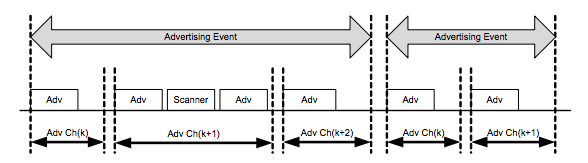
\includegraphics[width=0.5\linewidth]{2.Chapter/Advertising_event.png}
	\caption[Advertising event]{Advertising event}
	\label{fig:ad_event}
\end{figure}

\tab \textbf{Advertising events:} There are three roles that can be used to describe a device in function of their utilisation of the channel: \textbf{advertisers}, are those that transmit advertising packets; \textbf{scanners} are devices that receive advertising packets without the intention of connecting with the advertising device; \textbf{initiators} are devices that listen for connectable advertising packets in order to later initiate a connection.
Transmissions in the advertising channels occur in advertising events which always start with an advertiser sending a packet. Depending on the type of advertising packet, a scanner device may make a request to the advertiser which may be followed by a response from the advertiser, always on the same advertising \ac{PHY} channel. The advertising \ac{PHY} channel changes when the advertiser sends a new advertising packet. An advertising event can be terminated whenever the advertiser wants and when a new advertising event is created it will  occur in the first advertising \ac{PHY} channel. The whole process can be visualised in \ref{fig:ad_event}.

\begin{figure}[H]
	\centering
		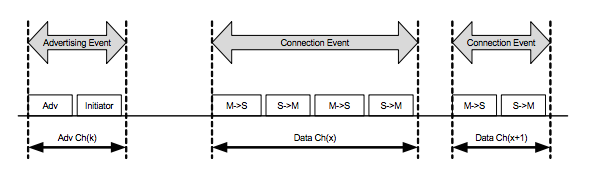
\includegraphics[width=0.5\linewidth]{2.Chapter/Conn_event.png}
	\caption[Connection Event]{Connection event}
	\label{fig:conn_event}
\end{figure}

\tab \textbf{Connection events:} When an advertiser is using a connectable advertising event an initiator may request a connection on the same \ac{PHY} channel. If the advertiser accepts the connection request, the advertising event ends and a connection event starts in order to establish the connection. Once it's established the initiator takes the master role and the advertised, the slave role. These events are used to transmit data between each other and they always begin with a message from the master. During a connection event master and slave alternate send data packets on the same packet. The master is responsible for ending the end whenever he pleases and for the creation of new event channel hopping is required. The whole connection event can be visualised in \ref{fig:conn_event}. 

\subsubsection{\ac{LE} Piconet Topology}
\label{subsec:piconet}

\begin{figure}[H]
	\centering
		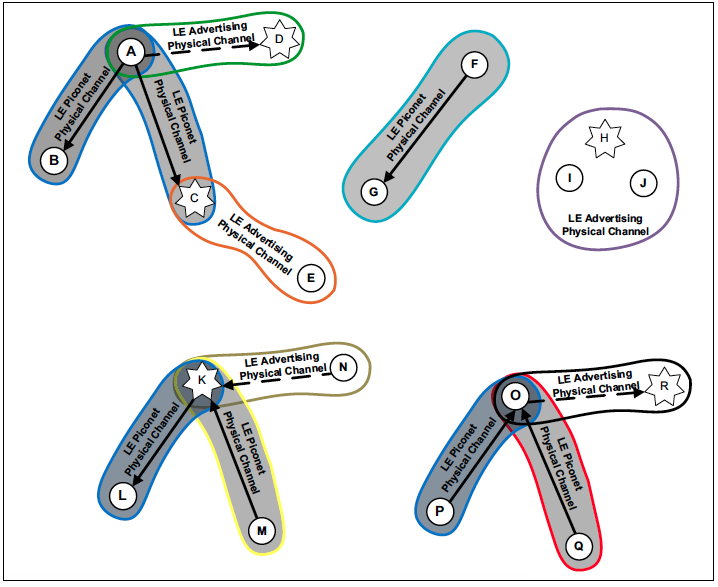
\includegraphics[width=0.5\linewidth]{2.Chapter/LEpiconet.png}
	\caption[LE Topology]{Examples of LE topology}
	\label{fig:LEpiconet}
\end{figure}

As opposed to regular Bluetooth piconet, in \ac{LE}, slaves can't share a \ac{PHY} channel and as such each must have his own \ac{PHY} channel to communicate with a master device. In order to best understand \ref{fig:LEpiconet}, solid arrows always point from master to slave, dashed arrows indicate a connection initiation where the arrow points form the initatior to the advertised using a connection event and devices that are advertising are indicated with a star. With these notes the different types of topologies can be analysed:

\begin{itemize}
\item In piconet A, that which contains device A, there are multiple types of topologies such as , device A having connections with multiple slaves and initiating a new one with device D which was advertising. It is also worth noting that the device E is functioning as a scanner listening to the advertiser device C.

\item In piconet F there is a simple master slave connection with device F as master and G as slave.

\item In Group H there are more than two devices in a single \ac{PHY} channel, such thing occurs since multiple devices can listen for advertisements on the same channel. In this case device H is functioning as an advertiser while I and J are scanners.

\item In scatternet K there is an example where device K functions as master in the connection with device L and as a slave in the connection with device M, at the same time.

\item In scatternet O there is an example where device O is functioning as a slave in both his connections with devices P and Q but it is still capable of forming a connection with R, where O will be the master.
\end{itemize}

\subsubsection{Operational Procedures}
\label{subsec:Operational}

The most common operational mode of a Bluetooth device is when he is connected and exchanging data with another Bluetooth device. Since Bluetooth is an ad-hoc wireless communications technology, i.e. decentralised type of wireless network, there are a number of operational procedures that enable piconets to be formed so that the subsequent communications can take place.

\begin{description}
\item [Device Filtering Procedure] Method used by controllers to reduce the number of devices requiring communication responses through the use of a "white list" located in the Link Layer that enumerates the devices that are allowed to communicate with the local device. This procedure allows the device reduce power consumption since it reduces the number of transmissions that it needs to make.

\item [Advertising Procedure] An advertiser utilises this procedure to perform unidirectional broadcasts to devices in the vicinity. The broadcast occurs without any need of connections and can be utilised to establish connections with nearby devices or to simple broadcast information to nearby scanner devices. This procedure includes the operations already described in advertising events in \ref{subsec:Communication}.

\item [Scanning Procedure] A scanner device utilises this procedure to listen to unidirectional broadcasts of user data sent by advertising devices. It is also capable of requesting additional user data by making a scan request as an answer on the same \ac{PHY} channel of the first broadcast. This procedure can be utilised while the device is connected to other \ac{LE} devices for as long as its connections requirements are maintained.

\item [Discovering Procedure] Bluetooth devices use the advertising procedure and scanning procedure to discover nearby devices, or to be discovered by devices in a given area, as such the discovery procedure is asymmetrical. A Bluetooth device that tries to find other devices in the vicinity can be called as a discovering device and will listen for devices advertising scannable advertising events. Devices that are available to be found and actively broadcast scannable advertising events are called discoverable devices. 

\item [Connecting Procedure] The connecting procedure is asymmetrical as it requires one of the devices to be utilise the advertising procedure and the other one the scanning procedure. The advertising procedure has the capability of being targeted which allows only the chosen device to respond.  The scanning procedure also has the capability of being target if the device discovers an advertising device and from there on out only listens for its advertisings. Upon receiving a connectable advertising event, it can initiate the connection by answering with a connection request.

\item [Connected Mode] Once the Connecting procedure is over the devices are physically connected to each other within a piconet. While in connected mode there is the possibility of changing the connection's properties such as data packet's length and for the device to utilise advertising ,scanning or discovery procedures.
\end{description}

